\documentclass[tikz,border=3mm]{standalone}
\usepackage{mathptmx,amsmath,amssymb}
\usepackage{pgfplots}\pgfplotsset{compat=1.18}
\usetikzlibrary{arrows.meta,positioning,shapes.geometric,shapes.misc,fit,calc,backgrounds,decorations.pathreplacing}
\definecolor{tdInk}{HTML}{1D2330}\definecolor{tdMuted}{HTML}{5D6678}\definecolor{tdLine}{HTML}{D9D5CA}
\definecolor{tdBlue}{HTML}{2457D6}\definecolor{tdGreen}{HTML}{17855A}\definecolor{tdAmber}{HTML}{B7791F}
\definecolor{tdRed}{HTML}{C8362F}\definecolor{tdPurple}{HTML}{7A4FD1}
\tikzset{>={Stealth[length=2.2mm]},
  card/.style={rounded corners=3pt,draw=#1!70!black,fill=#1!9,align=center,inner sep=4pt,font=\small},card/.default=tdBlue,
  pill/.style={rounded corners=6pt,draw=none,fill=#1,text=white,inner sep=3pt,font=\footnotesize\bfseries,align=center},pill/.default=tdBlue,
  lbl/.style={font=\footnotesize,text=tdMuted,align=center},
  arr/.style={->,thick,draw=tdMuted},
  ttl/.style={font=\small\bfseries,anchor=west}}
\begin{document}

%% D1 framework ------------------------------------------------------------
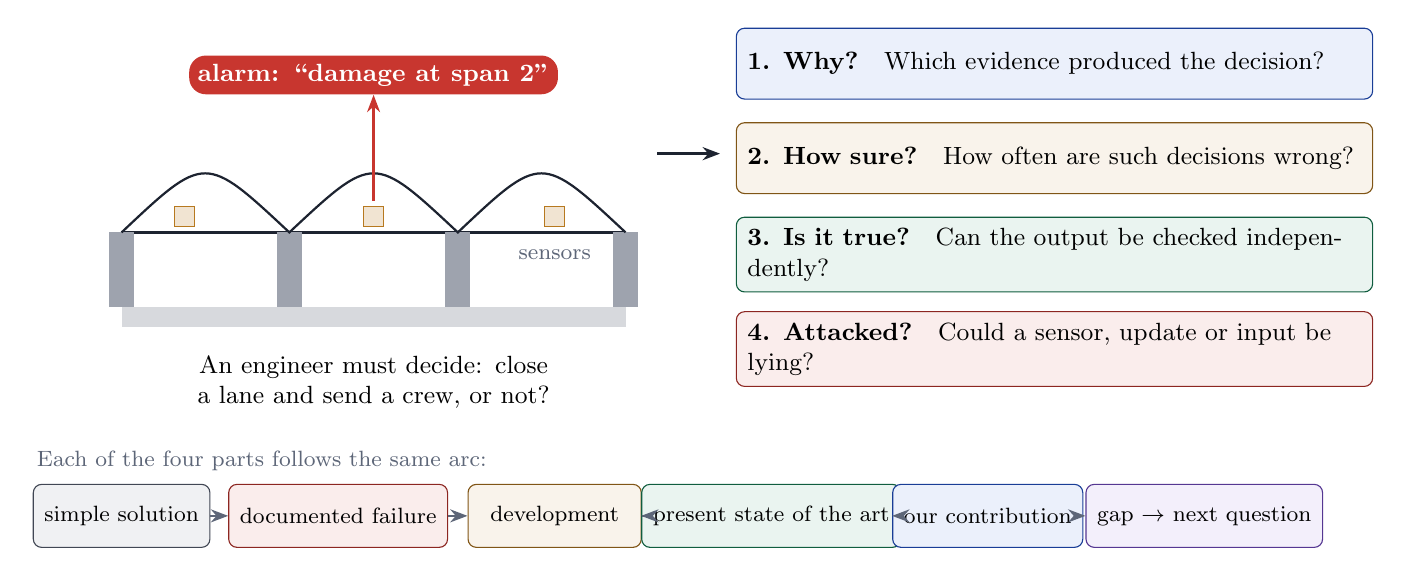
\begin{tikzpicture}[x=1mm,y=1mm]
  \fill[tdMuted!25] (0,0) rectangle (64,2.5);
  \draw[very thick,tdInk] (0,12) -- (64,12);
  \foreach \xx in {0,21.3,42.7,64}{\fill[tdMuted!60] (\xx-1.6,2.5) rectangle (\xx+1.6,12);}
  \draw[thick,tdInk] (0,12) .. controls (10.6,22) .. (21.3,12) .. controls (32,22) .. (42.7,12) .. controls (53.3,22) .. (64,12);
  \foreach \xx in {8,32,55}{\node[draw=tdAmber,fill=tdAmber!20,minimum size=2.6mm,inner sep=0] at (\xx,14) {};}
  \node[lbl,anchor=north] at (55,11) {sensors};
  \node[pill=tdRed,font=\small\bfseries] (al) at (32,32) {alarm: ``damage at span 2''};
  \draw[->,thick,tdRed] (32,16) -- (al.south);
  \node[font=\small,align=center,text width=60mm] at (32,-7) {An engineer must decide: close a lane and send a crew, or not?};
  \begin{scope}[xshift=78mm]
  \foreach \i/\q/\d/\c in {0/{1. Why?}/{Which evidence produced the decision?}/tdBlue,1/{2. How sure?}/{How often are such decisions wrong?}/tdAmber,2/{3. Is it true?}/{Can the output be checked independently?}/tdGreen,3/{4. Attacked?}/{Could a sensor, update or input be lying?}/tdRed}{
    \node[card=\c,text width=78mm,align=left,anchor=north west,minimum height=9mm] at (0,{38-\i*12}) {\textbf{\q}\quad \d};}
  \end{scope}
  \draw[->,very thick,tdInk] (68,22) -- (76,22);
  % story arc
  \begin{scope}[yshift=-24mm]
  \foreach \i/\t/\c in {0/{simple solution}/tdMuted,1/{documented failure}/tdRed,2/{development}/tdAmber,3/{present state of the art}/tdGreen,4/{our contribution}/tdBlue,5/{gap $\rightarrow$ next question}/tdPurple}{
     \node[card=\c,minimum width=22mm,minimum height=8mm,font=\footnotesize] (s\i) at ({\i*27.5},0) {\t};}
  \foreach \a/\b in {0/1,1/2,2/3,3/4,4/5}{\draw[arr] (s\a) -- (s\b);}
  \node[lbl,anchor=west] at (-12,7) {Each of the four parts follows the same arc:};
  \end{scope}
\end{tikzpicture}

%% D2 explain: (a) sanity check (b) heterophily ----------------------------
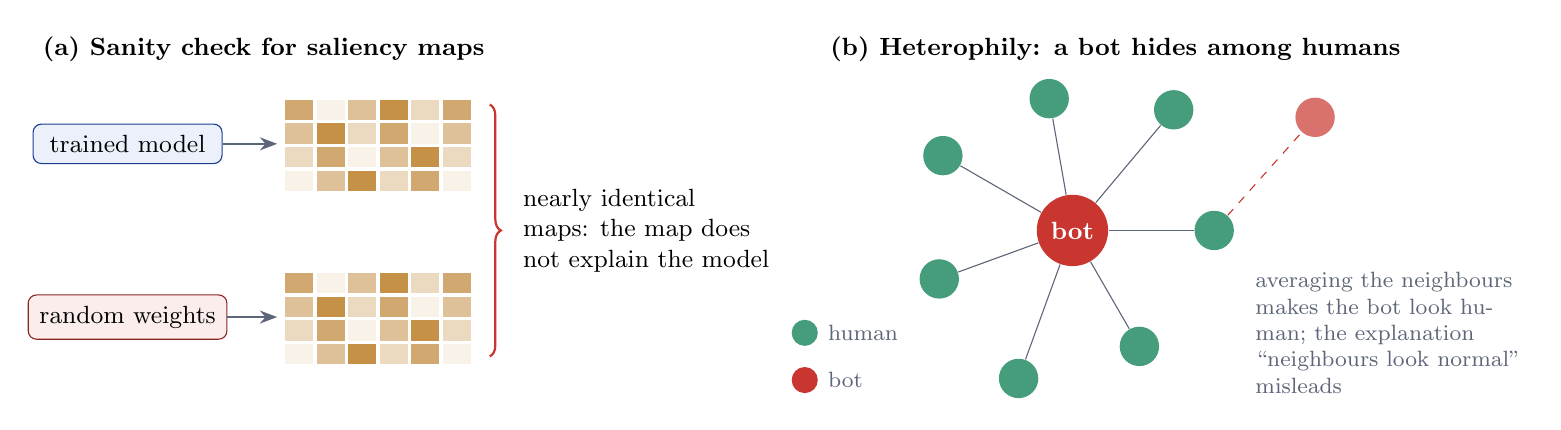
\begin{tikzpicture}[x=1mm,y=1mm]
  \node[ttl] at (-2,40) {(a) Sanity check for saliency maps};
  \node[card=tdBlue,minimum width=24mm] (m1) at (10,28) {trained model};
  \node[card=tdRed,minimum width=24mm] (m2) at (10,6) {random weights};
  \foreach \nn/\yy in {m1/28,m2/6}{
    \foreach \i in {0,...,5}{\foreach \j in {0,...,3}{
      \pgfmathsetmacro{\sh}{int(mod(\i*7+\j*11,5)*18+10)}
      \fill[tdAmber!\sh] (30+\i*4,\yy-6+\j*3) rectangle (33.6+\i*4,\yy-3.4+\j*3);}}
    \draw[arr] (\nn.east) -- (29,\yy);}
  \draw[tdRed,thick,decorate,decoration={brace,amplitude=4pt}] (56,33) -- (56,1);
  \node[font=\small,align=left,anchor=west] at (59,17) {nearly identical\\maps: the map does\\not explain the model};
  \begin{scope}[xshift=100mm]
  \node[ttl] at (-2,40) {(b) Heterophily: a bot hides among humans};
  \node[circle,fill=tdRed,text=white,font=\small\bfseries,minimum size=8mm] (b) at (30,17) {bot};
  \foreach \a/\r in {0/18,50/20,100/17,150/19,200/18,250/20,300/17}{
     \node[circle,fill=tdGreen!80,minimum size=5mm] (h\a) at ($(b)+(\a:\r mm)$) {};
     \draw[tdMuted] (b) -- (h\a);}
  \node[circle,fill=tdRed!70,minimum size=5mm] (b2) at ($(b)+(25:34mm)$) {};\draw[tdRed,dashed] (h0) -- (b2);
  \node[lbl,anchor=west,text width=34mm,align=left] at (52,4) {averaging the neighbours makes the bot look human; the explanation ``neighbours look normal'' misleads};
  \node[circle,fill=tdGreen!80,minimum size=3mm,label={[lbl]right:human}] at (-4,4) {};
  \node[circle,fill=tdRed,minimum size=3mm,label={[lbl]right:bot}] at (-4,-2) {};
  \end{scope}
\end{tikzpicture}

%% D3 XHBot ------------------------------------------------------------------
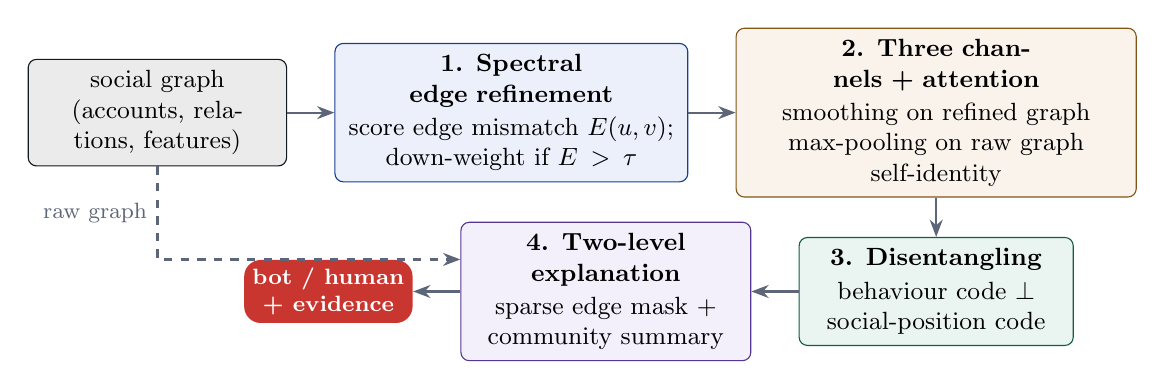
\begin{tikzpicture}[node distance=5mm and 6mm]
  \node[card=tdInk,text width=30mm] (g) {social graph\\ (accounts, relations, features)};
  \node[card=tdBlue,text width=42mm,right=of g] (s) {\textbf{1. Spectral edge refinement}\\[1pt] score edge mismatch $E(u,v)$;\\ down-weight if $E>\tau$};
  \node[card=tdAmber,text width=48mm,right=of s] (t) {\textbf{2. Three channels + attention}\\[1pt] smoothing on refined graph\\ max-pooling on raw graph\\ self-identity};
  \node[card=tdGreen,text width=32mm,below=of t] (c) {\textbf{3. Disentangling}\\[1pt] behaviour code $\perp$ social-position code};
  \node[card=tdPurple,text width=34mm,left=of c] (e) {\textbf{4. Two-level explanation}\\[1pt] sparse edge mask + community summary};
  \node[pill=tdRed,left=of e,minimum height=8mm] (o) {bot / human\\ + evidence};
  \draw[arr] (g) -- (s); \draw[arr] (s) -- (t); \draw[arr] (t) -- (c); \draw[arr] (c) -- (e); \draw[arr] (e) -- (o);
  \draw[arr,dashed] (g.south) |- (e.west|-o.north) node[pos=0.25,lbl,left]{raw graph};
\end{tikzpicture}

%% D4 split conformal --------------------------------------------------------
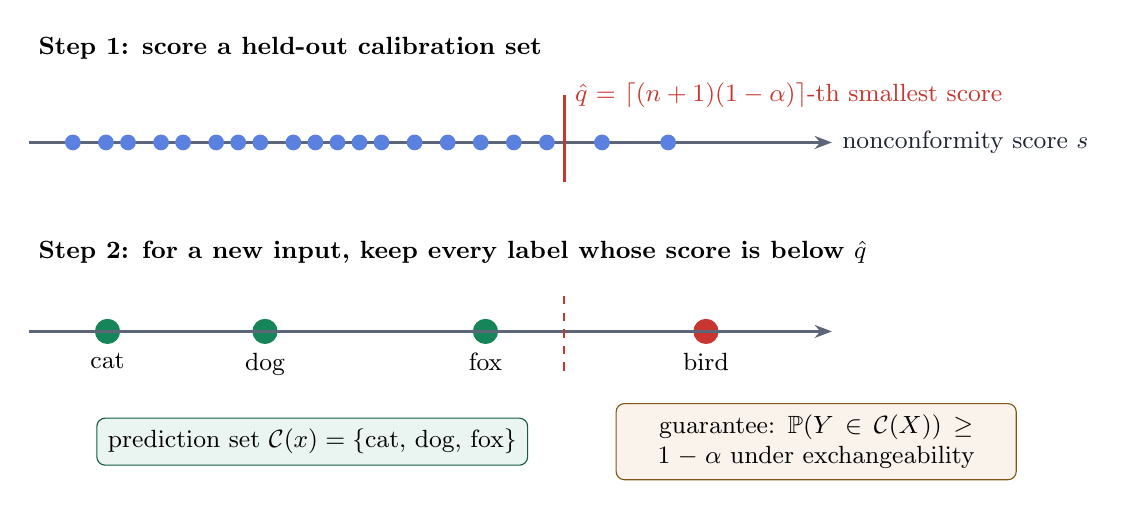
\begin{tikzpicture}[x=1mm,y=1mm]
  \node[ttl] at (0,32) {Step 1: score a held-out calibration set};
  \draw[->,thick,tdMuted] (0,20) -- (102,20) node[right,font=\small,text=tdInk] {nonconformity score $s$};
  \foreach \xx in {4,7,9,12,14,17,19,21,24,26,28,30,32,35,38,41,44,47,52,58}{\fill[tdBlue!75] (\xx*1.4,20) circle (1mm);}
  \draw[tdRed,very thick] (68,15) -- (68,26) node[right,font=\small,text=tdRed] {$\hat q$ = $\lceil (n+1)(1-\alpha)\rceil$-th smallest score};
  \node[ttl] at (0,6) {Step 2: for a new input, keep every label whose score is below $\hat q$};
  \foreach \xx/\nm/\cc in {10/cat/tdGreen,30/dog/tdGreen,58/fox/tdGreen,86/bird/tdRed}{\fill[\cc] (\xx,-4) circle (1.6mm);\node[font=\small,below=1.5mm] at (\xx,-4) {\nm};}
  \draw[->,thick,tdMuted] (0,-4) -- (102,-4);
  \draw[dashed,tdRed,thick] (68,-9) -- (68,1);
  \node[card=tdGreen,font=\small] at (36,-18) {prediction set $\mathcal C(x)=\{\text{cat, dog, fox}\}$};
  \node[card=tdAmber,font=\small,text width=48mm] at (100,-18) {guarantee: $\mathbb P(Y\in\mathcal C(X))\ge 1-\alpha$ under exchangeability};
\end{tikzpicture}

%% D5 verification: (a) formal (b) risk-coverage ----------------------------
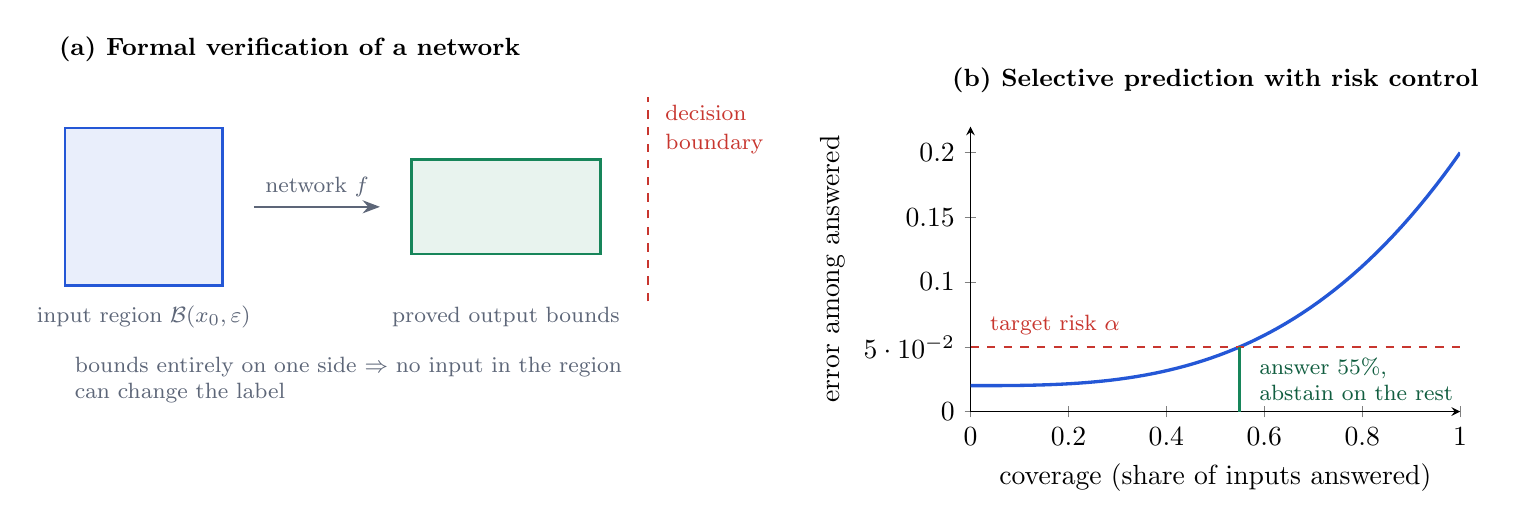
\begin{tikzpicture}
  \begin{scope}[x=1mm,y=1mm]
  \node[ttl] at (-2,34) {(a) Formal verification of a network};
  \draw[thick,tdBlue,fill=tdBlue!10] (0,4) rectangle (20,24); \node[lbl] at (10,0) {input region $\mathcal B(x_0,\varepsilon)$};
  \draw[->,thick,tdMuted] (24,14) -- (40,14) node[midway,above,lbl] {network $f$};
  \draw[thick,tdGreen,fill=tdGreen!10] (44,8) rectangle (68,20); \node[lbl] at (56,0) {proved output bounds};
  \draw[tdRed,dashed,thick] (74,2) -- (74,28); \node[lbl,text=tdRed,anchor=west] at (75,26) {decision};\node[lbl,text=tdRed,anchor=west] at (75,22) {boundary};
  \node[lbl,anchor=west,text width=70mm,align=left] at (0,-8) {bounds entirely on one side $\Rightarrow$ no input in the region can change the label};
  \end{scope}
  \begin{scope}[xshift=115mm,yshift=-12mm]
  \begin{axis}[width=7.8cm,height=5.2cm,xlabel={coverage (share of inputs answered)},ylabel={error among answered},xmin=0,xmax=1,ymin=0,ymax=0.22,axis lines=left,title={\small\bfseries (b) Selective prediction with risk control},title style={yshift=1mm}]
    \addplot[domain=0:1,samples=60,very thick,tdBlue] {0.02+0.18*x^3};
    \addplot[tdRed,dashed,thick] coordinates {(0,0.05)(1,0.05)};
    \addplot[tdGreen,very thick] coordinates {(0.55,0)(0.55,0.05)};
    \node[font=\footnotesize,text=tdRed,anchor=south west] at (axis cs:0.02,0.052) {target risk $\alpha$};
    \node[font=\footnotesize,text=tdGreen!70!black,anchor=west,align=left] at (axis cs:0.57,0.025) {answer 55\%,\\abstain on the rest};
  \end{axis}
  \end{scope}
\end{tikzpicture}

%% D6 CMVKG-Guard -----------------------------------------------------------
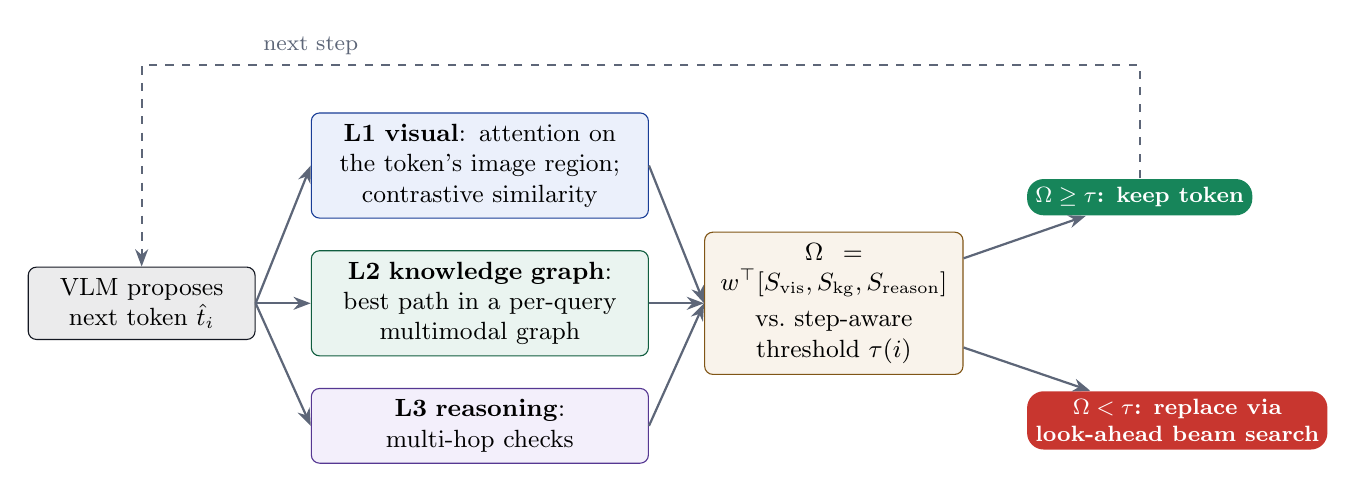
\begin{tikzpicture}[node distance=4mm and 7mm]
  \node[card=tdInk,text width=26mm] (v) {VLM proposes next token $\hat t_i$};
  \node[card=tdGreen,text width=40mm,right=of v] (l2) {\textbf{L2 knowledge graph}: best path in a per-query multimodal graph};
  \node[card=tdBlue,text width=40mm,above=of l2] (l1) {\textbf{L1 visual}: attention on the token's image region; contrastive similarity};
  \node[card=tdPurple,text width=40mm,below=of l2] (l3) {\textbf{L3 reasoning}: multi-hop checks};
  \node[card=tdAmber,text width=30mm,right=of l2] (o) {$\Omega=w^\top[S_{\mathrm{vis}},S_{\mathrm{kg}},S_{\mathrm{reason}}]$\\[2pt] vs.\ step-aware threshold $\tau(i)$};
  \foreach \l in {l1,l2,l3}{\draw[arr] (v.east) -- (\l.west); \draw[arr] (\l.east) -- (o.west);}
  \node[pill=tdGreen,above right=2mm and 8mm of o,minimum width=26mm] (k) {$\Omega\ge\tau$: keep token};
  \node[pill=tdRed,below right=2mm and 8mm of o,minimum width=26mm] (c) {$\Omega<\tau$: replace via\\ look-ahead beam search};
  \draw[arr] (o) -- (k); \draw[arr] (o) -- (c);
  \draw[arr,dashed] (k.north) |- ([yshift=6mm]l1.north) -| (v.north) node[pos=0.25,above,lbl] {next step};
\end{tikzpicture}

%% D7 FL + FORTRESS ---------------------------------------------------------
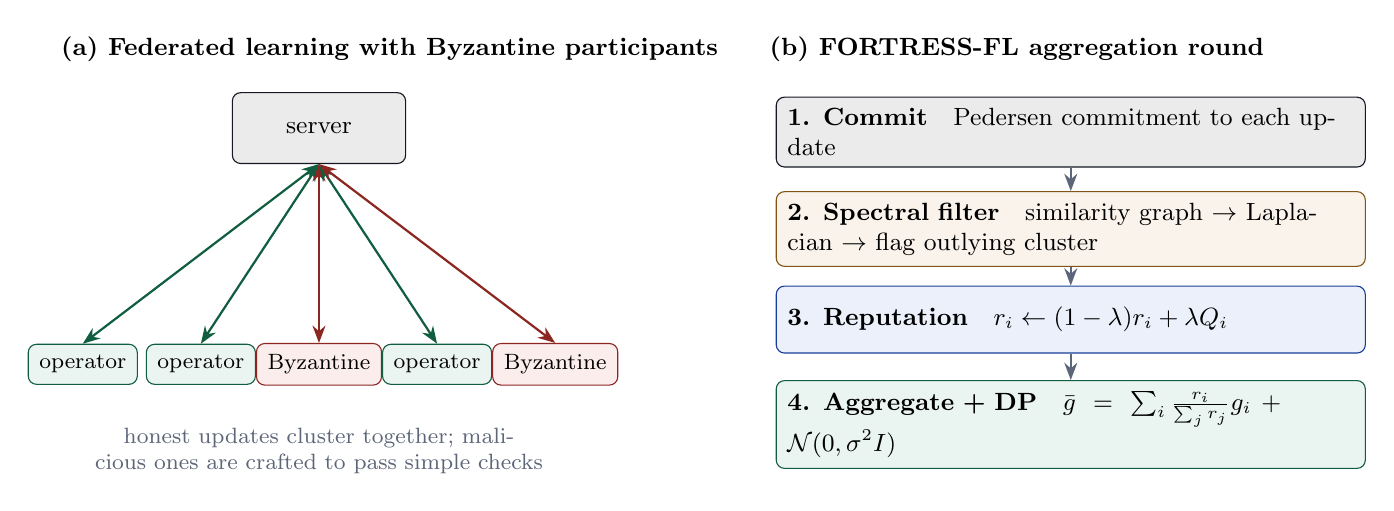
\begin{tikzpicture}[x=1mm,y=1mm]
  \node[ttl] at (-4,48) {(a) Federated learning with Byzantine participants};
  \node[card=tdInk,minimum width=22mm,minimum height=9mm] (srv) at (30,38) {server};
  \foreach \i/\c/\t in {0/tdGreen/{operator},1/tdGreen/{operator},2/tdRed/{Byzantine},3/tdGreen/{operator},4/tdRed/{Byzantine}}{
    \node[card=\c,minimum width=13mm,font=\footnotesize] (c\i) at ({\i*15},8) {\t};
    \draw[<->,thick,\c!70!black] (c\i.north) -- (srv.south);}
  \node[lbl,text width=70mm] at (30,-3) {honest updates cluster together; malicious ones are crafted to pass simple checks};
  \begin{scope}[xshift=88mm]
  \node[ttl] at (-2,48) {(b) FORTRESS-FL aggregation round};
  \foreach \i/\c/\t/\d in {0/tdInk/{1. Commit}/{Pedersen commitment to each update},1/tdAmber/{2. Spectral filter}/{similarity graph $\rightarrow$ Laplacian $\rightarrow$ flag outlying cluster},2/tdBlue/{3. Reputation}/{$r_i\leftarrow(1-\lambda)r_i+\lambda Q_i$},3/tdGreen/{4. Aggregate + DP}/{$\bar g=\sum_i \frac{r_i}{\sum_j r_j}g_i+\mathcal N(0,\sigma^2 I)$}}{
     \node[card=\c,text width=72mm,align=left,anchor=north west,minimum height=8.5mm] (f\i) at (0,{42-\i*12}) {\textbf{\t}\quad \d};}
  \foreach \a/\b in {0/1,1/2,2/3}{\draw[arr] (f\a.south) -- (f\b.north);}
  \end{scope}
\end{tikzpicture}

%% D8 VOUCH -----------------------------------------------------------------
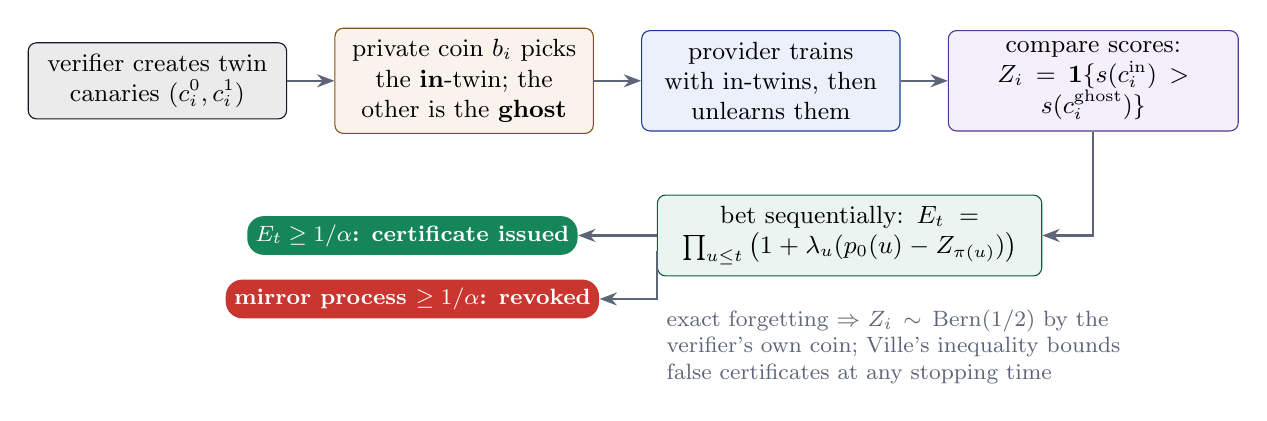
\begin{tikzpicture}[node distance=4mm and 6mm]
  \node[card=tdInk,text width=30mm] (tw) {verifier creates twin canaries $(c_i^0,c_i^1)$};
  \node[card=tdAmber,text width=30mm,right=of tw] (coin) {private coin $b_i$ picks the \textbf{in}-twin; the other is the \textbf{ghost}};
  \node[card=tdBlue,text width=30mm,right=of coin] (ft) {provider trains with in-twins, then unlearns them};
  \node[card=tdPurple,text width=34mm,right=of ft] (z) {compare scores:\\ $Z_i=\mathbf 1\{s(c^{\mathrm{in}}_i)>s(c^{\mathrm{ghost}}_i)\}$};
  \node[card=tdGreen,text width=46mm,below=8mm of ft,xshift=10mm] (bet) {bet sequentially: $E_t=\prod_{u\le t}\big(1+\lambda_u(p_0(u)-Z_{\pi(u)})\big)$};
  \node[pill=tdGreen,left=10mm of bet,minimum width=30mm] (iss) {$E_t\ge 1/\alpha$: certificate issued};
  \node[pill=tdRed,below=3mm of iss,minimum width=30mm] (rev) {mirror process $\ge 1/\alpha$: revoked};
  \foreach \a/\b in {tw/coin,coin/ft,ft/z}{\draw[arr] (\a) -- (\b);}
  \draw[arr] (z.south) |- (bet.east); \draw[arr] (bet) -- (iss); \draw[arr] (bet.west) ++(0,-2mm) |- (rev.east);
  \node[lbl,text width=60mm,align=left,anchor=north west] at ([yshift=-3mm]bet.south west) {exact forgetting $\Rightarrow$ $Z_i\sim\mathrm{Bern}(1/2)$ by the verifier's own coin; Ville's inequality bounds false certificates at any stopping time};
\end{tikzpicture}

%% D9 Agents + CAPS -----------------------------------------------------------
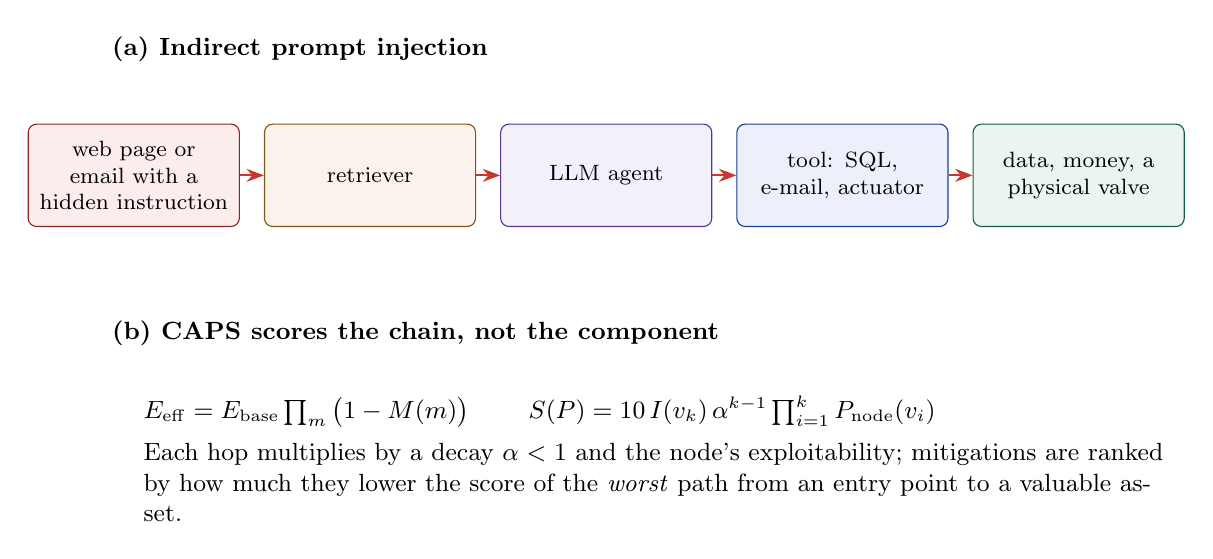
\begin{tikzpicture}[x=1mm,y=1mm]
  \node[ttl] at (-4,40) {(a) Indirect prompt injection};
  \foreach \i/\c/\t in {0/tdRed/{web page or email with a hidden instruction},1/tdAmber/{retriever},2/tdPurple/{LLM agent},3/tdBlue/{tool: SQL, e-mail, actuator},4/tdGreen/{data, money, a physical valve}}{
    \node[card=\c,text width=24mm,minimum height=13mm,font=\footnotesize] (p\i) at ({\i*30},24) {\t};}
  \foreach \a/\b in {0/1,1/2,2/3,3/4}{\draw[->,thick,tdRed] (p\a) -- (p\b);}
  \node[ttl] at (-4,4) {(b) CAPS scores the chain, not the component};
  \node[font=\small,anchor=west] at (0,-6) {$E_{\mathrm{eff}}=E_{\mathrm{base}}\prod_m\big(1-M(m)\big)$ \qquad $S(P)=10\,I(v_k)\,\alpha^{k-1}\prod_{i=1}^{k}P_{\mathrm{node}}(v_i)$};
  \node[font=\small,anchor=west,text width=130mm,align=left] at (0,-15) {Each hop multiplies by a decay $\alpha<1$ and the node's exploitability; mitigations are ranked by how much they lower the score of the \emph{worst} path from an entry point to a valuable asset.};
\end{tikzpicture}

%% D10 synthesis -----------------------------------------------------------
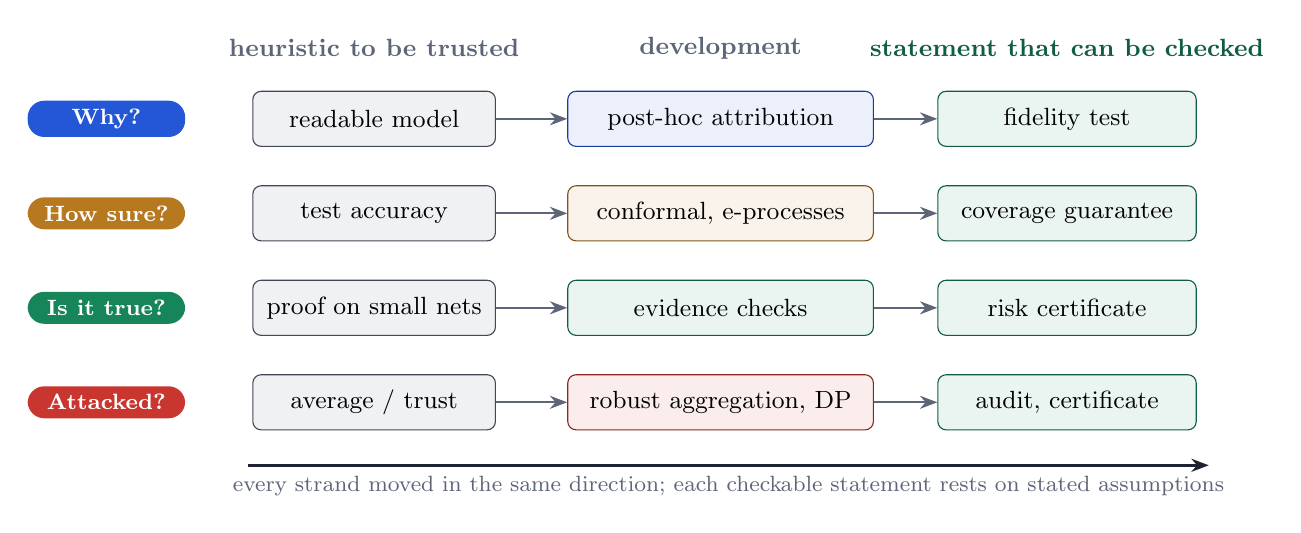
\begin{tikzpicture}[x=1mm,y=1mm,font=\small]
  \foreach \yy/\cc/\q/\simple/\now/\check in {
     36/tdBlue/{Why?}/{readable model}/{post-hoc attribution}/{fidelity test},
     24/tdAmber/{How sure?}/{test accuracy}/{conformal, e-processes}/{coverage guarantee},
     12/tdGreen/{Is it true?}/{proof on small nets}/{evidence checks}/{risk certificate},
     0/tdRed/{Attacked?}/{average / trust}/{robust aggregation, DP}/{audit, certificate}}{
    \node[pill=\cc,minimum width=20mm] at (0,\yy) {\q};
    \node[card=tdMuted,text width=28mm,minimum height=7mm] (a) at (34,\yy) {\simple};
    \node[card=\cc,text width=36mm,minimum height=7mm] (b) at (78,\yy) {\now};
    \node[card=tdGreen,text width=30mm,minimum height=7mm] (c) at (122,\yy) {\check};
    \draw[arr] (a) -- (b); \draw[arr] (b) -- (c);}
  \node[font=\small\bfseries,text=tdMuted] at (34,45) {heuristic to be trusted};
  \node[font=\small\bfseries,text=tdMuted] at (78,45) {development};
  \node[font=\small\bfseries,text=tdGreen!70!black] at (122,45) {statement that can be checked};
  \draw[->,line width=1.2pt,tdInk] (18,-8) -- (140,-8) node[midway,below,lbl] {every strand moved in the same direction; each checkable statement rests on stated assumptions};
\end{tikzpicture}
\end{document}
